%% Languages: norsk				
%%						english			
%% Styles:		twoside, 		The margins will differ dependent on right/left pages
%%						openright		The first page is a "right" page
%%  indexes:		listings		Show figure list, table list
%%						glossary		Show glossary and abbreviation list
%%						todo				Show list of todo-notes in documents
%%						%
\documentclass[english]{gucreport}
\projdate{ \today }
\projvers{ 1.0 }

\courseid{ IMT3521 }
\coursename{  Security Planning and Incident Management }
\projteacher{ Marie Elisabeth Gaup Moe }

\appnumber{ N/A } %	number of appendixes
								%	currently auto calculated but might be wrong
\pagecount{ \pageref{LastPage} }

\projtitle{ Smoking Games }
\projsubtitle{ Contingency Plan }

\projauthor{ Adrián Alberdi Ainziburu }
\projauthorid{ 130197 }
\projauthorA{ Leonard Eschenbaum }
\projauthorAid{ 131721 }
\projauthorB{ }
\projauthorBid{ }
\projauthorC{ }
\projauthorCid{ }
\projauthorD{ }
\projauthorDid{ }

%\renewcommand{\familydefault}{\sfdefault}
%\rmfamily

\begin{document}
	%%%
%%	Dictonary
%%		\newglossaryentry{unique_id}{name={Term}, description={Description}}
%%
%\newglossaryentry{}{name={}, description={}}
\newglossaryentry{lorem}{name={Lorem ipsum}, description={AKSJDKLAJSLKD 12"/(/}}

%%
%%	Abbreviations
%%		\nomenclature{Abbreviation}{Description}
%%
%\nomenclature{}{}
\nomenclature{OS}{Operating System}
\nomenclature{LTS}{Long Term Support}
\nomenclature{ROTFWLMAO}{Rolling On The Floor While Laughing My Ass Off}


	\makefrontpages
	\tableofcontents
	\showindex		%%lists of figures, codes, tables, glossary, etc
	
	%% Chapters for the text
	\chapter{Business description}
Smoking games was founded in 2008 by a group of 5 international students. The founders met at guc during
the 1st semester of 2008. \\
This enterprise produces and digitally distributes games. The enterprise is located in Tenerife, Spain.
\section{Business Overview}
Smoking Games started as a small video game developer. At the beginning they distributed their games through other distributers. After the great hit of a video game called ''full life'', they decided to start distributing their games on their own.\\
In 2010, after 2 years in the development business, Smoking Games became a video game developer and digital distributor company. At the start they only distributed their own games. With the growth of the enterprise, Smoking Games got many offers from other game developers to distribute their games. Smoking Games decided, that they will distribute also other developers's creations in their digital distribution section. At this point the distribution software, which is free for download for users, was named "Smoke".\\
2011 was a great year for Smoking Games: the growth of computer gaming helped consolidating the enterprise and Smoke became the distribution and gaming platform for everyone. In Smoking Games they didn't think it was enough, as their mission states: "Always creating and innovating". So they took the next step, a cloud service for saving games and cross platform gaming. Playing on two devices always moving forward in a shared game. Also, ''full life 3'' was released during this year, giving Smoking Games a very good position in the market as a trusted game developer.\\
In 2012, after 4 years in a rented placement, the headquarter of Smoking Games moved to a newly owned location. Taking advantage of this growth the whole enterprise grew. It redefined in this year still at the same size of 35 employees fixed plus some external services. Even though the enterprise organization is quite horizontal, the shares and benefits belong to the employees and bosses in the same amount, they keep a minimal organization for political purposes. The hierarchy of the enterprise is shown in figure \ref{fig:org_hierarchy}.

\begin{figure}[htpb]\centering
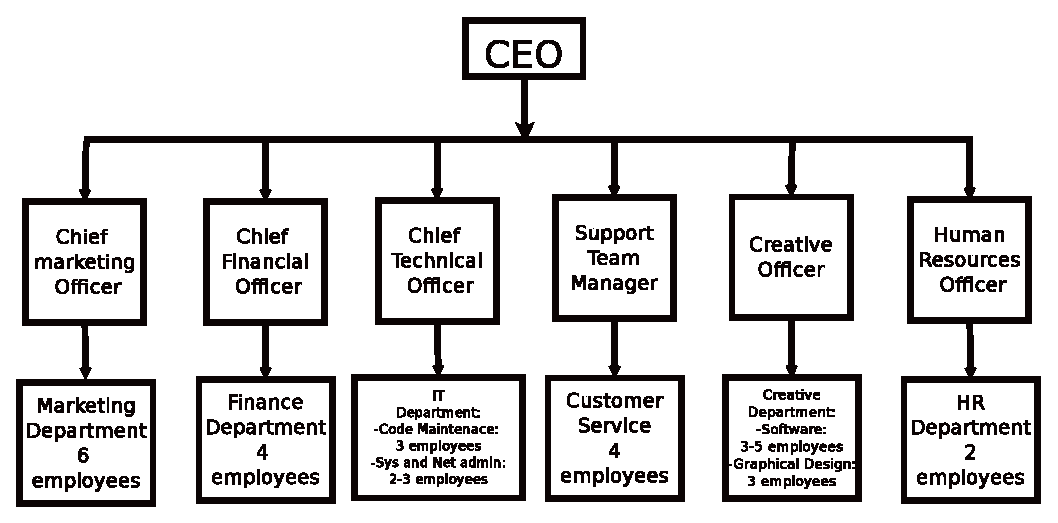
\includegraphics[ width={0.7\textwidth} ] {pictures/Organizational_hierarchy}
\caption{Organizational hierarchy}
\label{fig:org_hierarchy}
\end{figure}
\newpage
\noindent The main source of income for Smoking Games is selling their own games. These sales give a 100\% of the price back. The games produced by other companies are a different story: for every game and developer Smoking Games makes a different contract, going from the 75 to the 50\% money of the sales in the distribution price.\\
Smoking Games is located in a building in Tenerife, Spain. The building next to it is one of the main hubs for telefonica SA, main internet company in Spain. Like this the internet conection is much more ensured. This is important because most of Smoking Games's business is done over the internet.

\chapter{Assets}
Smoking Games' assets can be categorized into tangible and intangible assets. Every service consulted or used by Smoking Games which benefits them or is more or less essential for business processes is considered an asset.
\section{Tangible Assets}
Besides the obvious assets like building, computers or other hardware, power, water and data and telecommunication services are essential for Smoking Games' business processes and procedures and are therefore considered an asset because when one of these services is not available anymore it will inflict damage on their business economy. All tangible assets are shown in table \ref{tab:TangibleAssets}
\begin{center}
	\begin{tabular}{l | l}\label{tab:TangibleAssets}
		\textbf{Asset} & \textbf{Economic Benefit}\\\hline\hline
		Office Building and Offices & Provides space for employees\\\hline
		Office Equipment & \parbox[t]{7cm}{Provides the necessary equipment\\for employees}\\\hline
		in-house IT-system \& File Storage & \parbox[t]{7cm}{Provides maintainability and storage\\of customer information\\and applications}\\\hline
		Server Farm & \parbox[t]{7cm}{Provides accessibility for customers\\and employees}\\\hline
		Other Machines & Used for the production of goods\\\hline
		Other Hardware & \parbox[t]{7cm}{Used for different business processes}\\\hline
		Access Control & \parbox[t]{7cm}{Provides selective restriction of access\\to resources}\\\hline
		\parbox[t]{7cm}{External Security Services\\(e.g. security guard, alarm system, CCTV cameras)} & \parbox[t]{7cm}{Provides protection of other assets\\or people}\\\hline
		Emergency Generator & Provides backup power\\\hline
		\parbox[t]{8cm}{Data and Telecommunication,\\Power \& Water Services} & \parbox[t]{7cm}{Provides essential accessibility for\\business processes}\\\hline
		Renovation & \parbox[t]{7cm}{Provides maintainability of e.g. buildings}\\
	\end{tabular}
\end{center}
\section{Intangible Assets}

\section{Business Procedures and Processes}

%%\subsection{Risk management process}



\subsection{Internal procedures}
The main internal procedure is the game creation. Besides this, as any other enterprise there are different internal procedures, human resources and IT maintenance, for example. The game creation follows the procedure shown in the figure \ref{fig:proc_game_creation} and is the following:

\begin{figure}[h] \centering
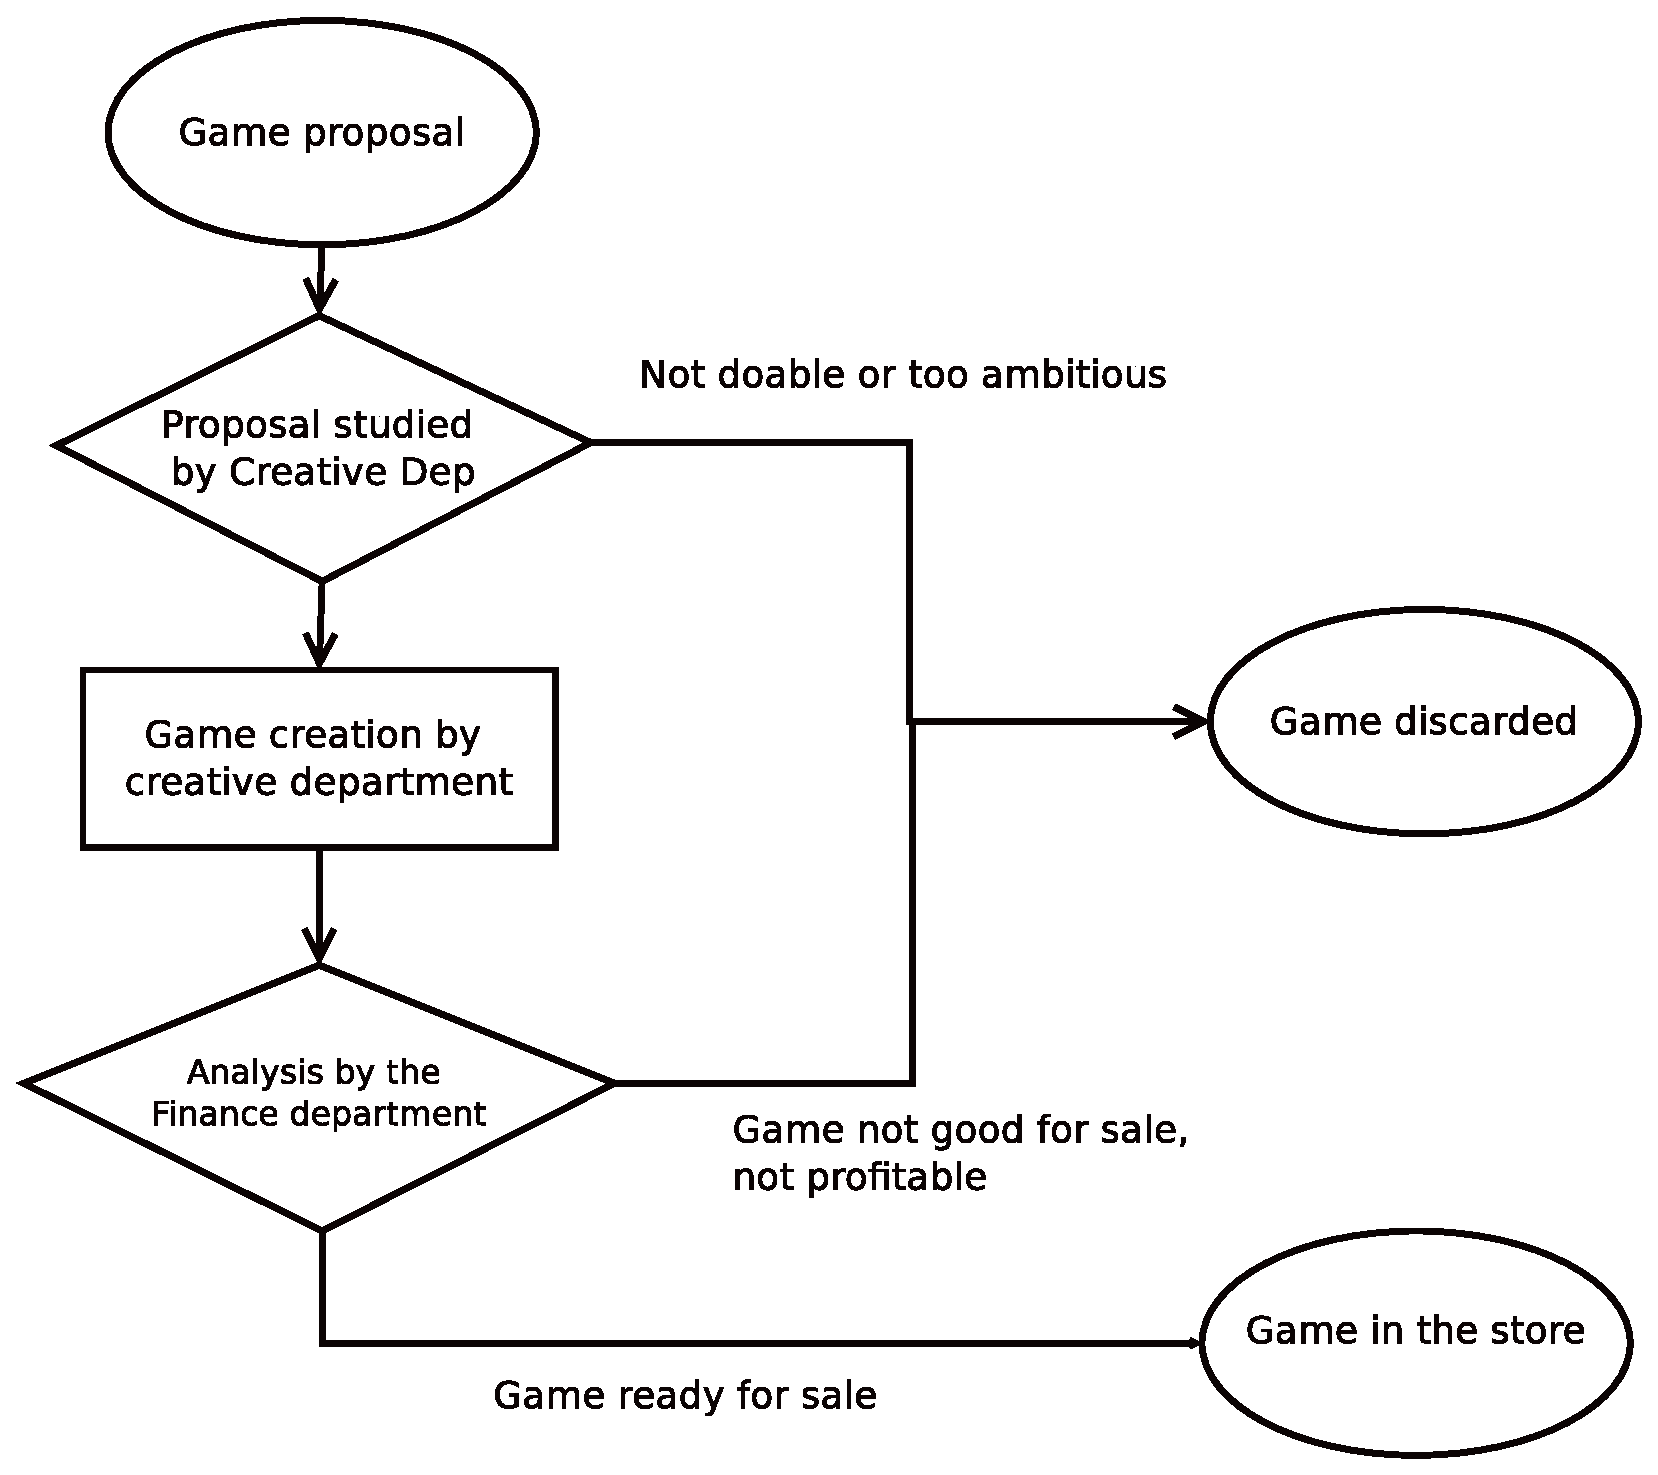
\includegraphics[width={0.7\textwidth}]{pictures/game_creation_process.eps}
\caption{Game creation process}
\label{fig:proc_game_creation}
\end{figure}

\begin {description}
\item{Idea creation: }This is the longer stage. It is a constant work in progress, during any stage the new ideas are taken in account. Once one project is finished a new idea is taken from the database.
\item{Idea study: }At this stage the idea is studied to check if it is doable, profitable and innovative. If it doesn't give the expected results the game idea is discarded.
\item{Game creation: }In this state the creative department starts the development of the project on itself. The development starts by programing the basic physics, story and the base program in general. When the 30\% of the estimated program is coded the design team starts working. At this early stage all the design is prepared for advertisement. While the game develops and the first alphas are launched the designers work more in the general graphics of the game.
\item{Game analysis: }When the game is around the 60\% through the development it's examined by the marketing department. If it gives clues for good and profitable sales it's approved and a marketing campaign is launched. If the game doesn't look good 	enough it's discarded.
\end {description}

\subsection{External procedures}
The main external procedure of Smoking games is the negotiation and signature of contracts with third party developers.

\begin{figure}[h]\centering
\includegraphics[ width={0.7\textwidth}]{pictures/third_party_game_process.eps}
\caption{Process for third party game distribution approval}
\label{fig:proc_third_party}
\end{figure}

This process as shown on the figure \ref{fig:proc_third_party} the process for signing a new contract is:

\begin{description}
\item{Project proposal reception: }The new game project is received in Smoking Games HQ.
\item{Project proposal analysis: }The project is given to the marketing department for market acceptance analysis and profit analysis. The marketing department will see the profitability of the project. In case the project doesn't give back a minimum the project will be discarded, and the developer told.
\item{Contract creation: }at this step the finance department will create a contract to present to the developer. The initial conditions of this contract have to have some flexibility for being able to negotiate. 
\item{Negotiation: }This newly created contract is presented and negotiated with the game developer. Depending on the result of this negotiation the project will be discarded or signed and validated.
\end{description}



An also important external procedure is the games sale through Smoke. This procedure is done using different payment options, credit card, pay pal or amazon payments, for example.
\newpage
\section{Network and Security}
To provide their customers security regarding their information, Smoking Games maintain their own in-house IT-system and file storage. This also gives the employees easy access to customer information with respect to the C.I.A. principles (confidentiality, integrity, availability).
\subsection{Network}
Smoking Games host their own Web services. Maintenance of these services and the rest of the network is the responsibility of Smoking Games' own IT department.\\
The company network is divided in, roughly speaking, three parts: the public network (DMZ), the internal network and the wireless network. An overview of the network topology is shown in figure \ref{fig:net_top}.\\
All connections between the outside and the internal network or the DMZ are being filtered by the external router which has a firewall included. The DMZ (demilitarized zone) contains public services such as a Web server or a VPN server (used for e.g. consulting purposes). Access to these services is restricted and handled by, as mentioned, the external router, which is configured to route packets between the outside and the DMZ differently than between the outside and the internal network. Additionally and IDS/IPS (incident detection/incident prevention system) is placed between the public network and the external router.\\
In case of a compromised external router all connectios between the outside and the internal network are being protected by an IDS/IPS and an internal router, which has additional filer lists implemented.\\
All information and data about customers or other business aspects are stored on the database server and file storage, respectively. Access to this data is handled by a router with a strictly configured firewall, so to avoid unauthorized access.\\
The rest of the internal network consists of work machines and a print server and printer.\\
A wireless network is also being provided, but it is not connected to the other network to avoid that information about customers or business projects is being stored on personal mobile devices.
\begin{figure}[h]\centering
	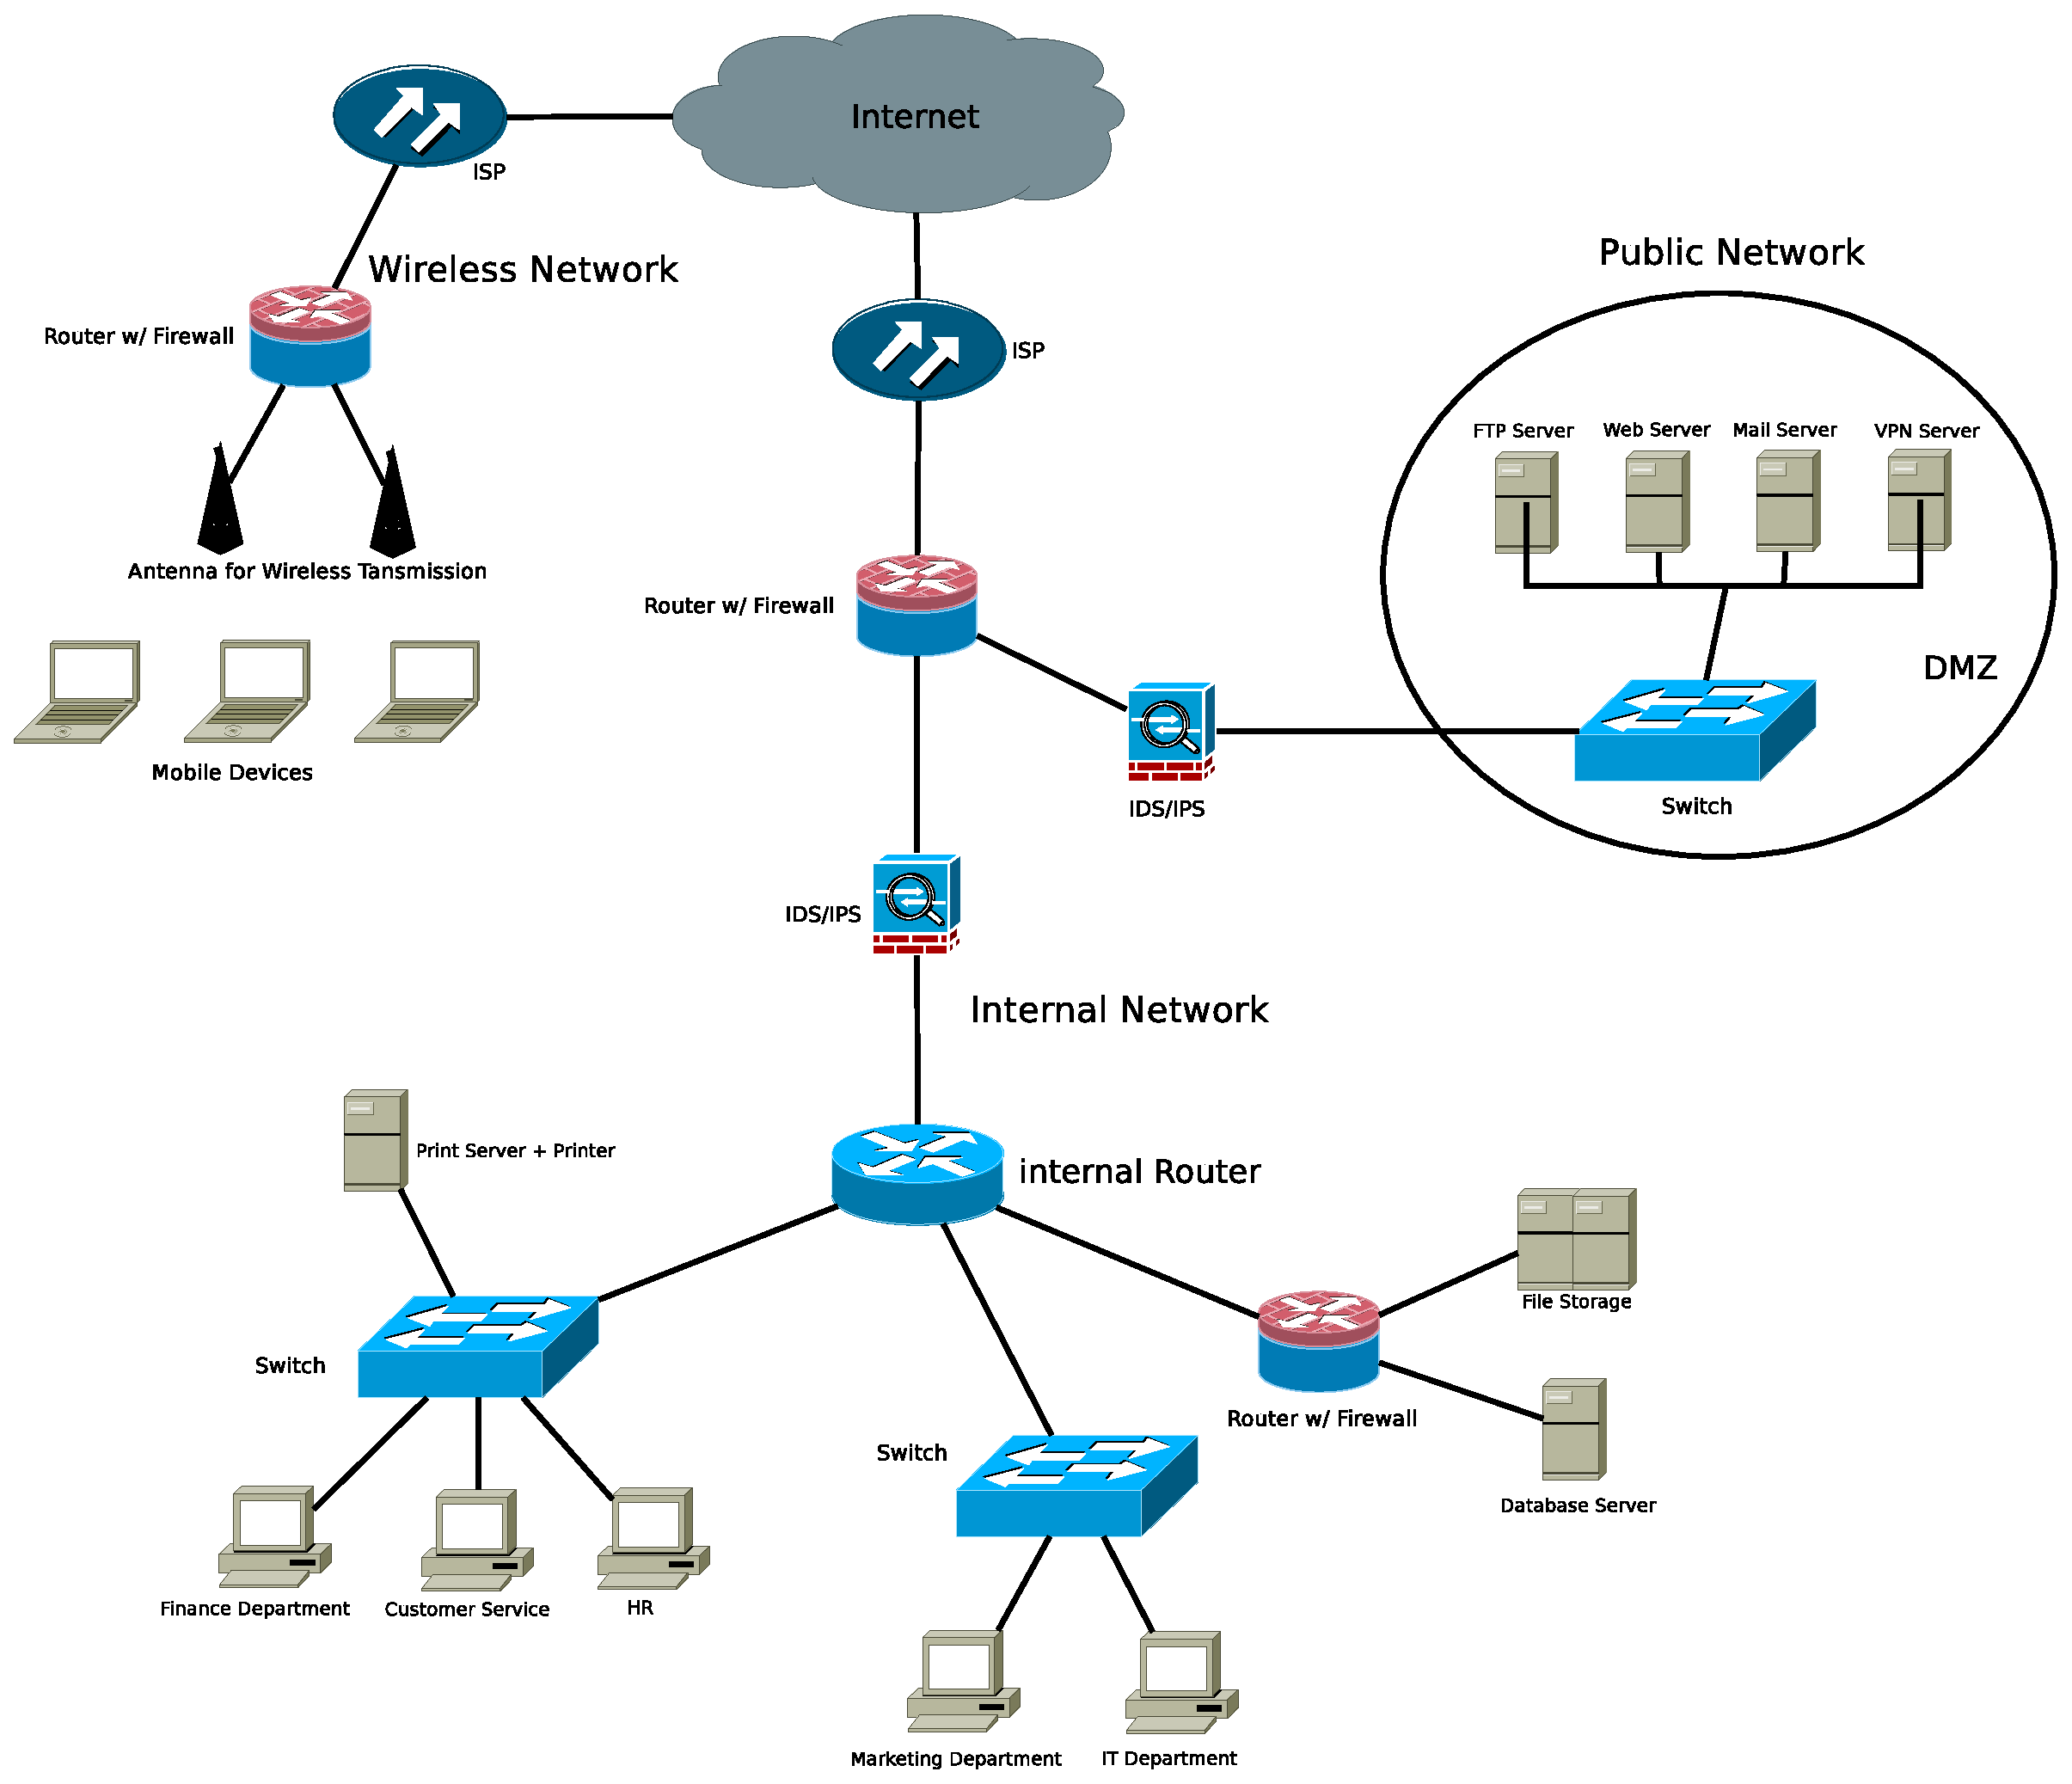
\includegraphics[scale=.3]{pictures/network_topology.eps}
	\caption{Network Topology}
	\label{fig:net_top}
\end{figure}
\subsection{Rules and Regulation}
As BYOD (bring your own device) is becoming more and more a security risk for companies, Smoking Games have strict policies for personal mobile devices. They are only allowed to use in the wireless area and (of course) outside the company network. Also, no information regarding the customers or business projects is allowed to keep or use on the devices. Flash drives provided by Smoking Games are encrypted and have an installed anti-spyware protable scanner to keep them free of malware. They are allowed to use inside the companies network, but not in the wireless area or outside of the building. The same applies for other mobile devices provided by Smoking Games.\\
All employees are required to properly secure their work equipment as a part of the employee contract they have signed with the company. In return the company promises to give adequate education on how to secure their equipment. This kind of security measures includes anti-virus,
secure communication, physical security, clear-desk policy and other relevant topics. Also, the security team has to make sure, that on every machine the latest security updates are installed.\\
Smoking Games have an incremental daily backup strategy and a complete back-up each Friday night. These back-ups are stored both on site and off site. The off site storage facility is a third party service provider, which complies with the same policies and legislative demands as Smoking Games.\\


	\chapter{Business Impact Analysis}
The business impact analysis (BIA) is divided into five parts\cite{whitman1}. The first part deals with the analysis of the risk each threat poses to Smoking Games (see \ref{sec:IdentThreatsAttacks}). Following from this, the Business Unit Analysis (BUA) is being performed, which indicates how the business would suffer under the loss of a business function --ref--. In part three different scenarios of successful attacks are being discussed --ref--. From these attack scenarios, in part four, the costs of the best, worst and moste likely outcomes is being estimated --ref--. Finally, in part five the attack scenarios are being classified according to severity to determine which subordinate plan should deal with it --ref--.


\section{Identification of Threats and Attacks}\label{sec:IdentThreatsAttacks}
In this section the list of threats discovered in the risk identification process\ref{RiskIdent} is being converted into a prioritized list of attacks. For this a Weighted Business Risk Analysis (WBRA) is being performed: the threats are weighted with a 50-50 split between probability and consequence, though consequence is divided into damage cost (30\%) and repair cost (20\%). Each threat scenario is followed by a short discription, which gives an explanation about the weights that are given. It is arranged by the "Total" value (from high to low). Prioritization of each scenario is based upon which resources are most valuable to the company. Preservation of human lifes is always prioritized.\\
Table \ref{ref:tabWBRA} shows the results of the WBRA and is derived from table 2-2 \cite{whitman2}.\\
\begin{longtable}{| p{4.2cm} | p{1.8cm} | p{1.8cm} | p{1.8cm} | p{1.8cm} |}
		\caption{Weighted Business Risk Analysis}\label{ref:tabWBRA}\\
		%the following until endfirsthead goes on top of table on first page
		\hline \multicolumn{5}{|c|}{\textbf{Weighted Business Risk Analysis}}\\\hline
		\textbf{Threat} & \textbf{Probability (0.5)} & \textbf{Damage Cost (0.2)} & \textbf{Repair Cost (0.3)} & \textbf{Total (1.0)}\\\hline
		\endfirsthead
		%the following until endhead goes on top of table of every page except first page
		\textbf{Threat} & \textbf{Probability (0.5)} & \textbf{Damage Cost (0.2)} & \textbf{Repair Cost (0.3)} & \textbf{Total (1.0)}\\\hline
		\endhead
		%the following until endfoot goes at bottom of table except last page
		\multicolumn{5}{|c|}{\textit{continued on next page}}\\
		\endfoot
		%the following until endlastfoot goes at bottom of table on last page
		\endlastfoot
		Fire & 0.5 & 0.9 & 0.8 & 0.67\\\hline
		& \multicolumn{4}{|p{8cm}|}{\textit{The likelihood for a fire to occur is moderate because of the mostly warm weather; the damage cost is very high; the repair cost is high, because equipment or building parts need to be repaired.}}\\\hline
		Denial of service attack & 0.7 & 0.8 & 0.5 & 0.66\\\hline
		& \multicolumn{4}{|p{8cm}|}{\textit{Very likely to happen; would cause high damage, because customers/users won't have access to the servers.}}\\\hline
		Social engineering attack via e-mail & 0.8 & 0.6 & 0.4 & 0.64\\\hline
		& \multicolumn{4}{|p{8cm}|}{\textit{Very likely that some phishing e-mails will go through the spam-filter, but it would most likely cause minimal damage because of routines.}}\\\hline
		Information leakage & 0.5 & 0.8 & 0.8 & 0.63\\\hline
		& \multicolumn{4}{|p{8cm}|}{\textit{High damage and high risk. It also has a high cost because it is difficult to discover and most likely not fixable.}}\\\hline
		Strong winds & 0.7 & 0.5 & 0.6 & 0.63\\\hline
		& \multicolumn{4}{|p{8cm}|}{\textit{Likely to occur; the damage cost is moderate due to the fact Smoking Games does not have any assets exposed other than it may be temporary loss of third party services; the repair cost is also moderate since building damage needs to be repaired.}}\\\hline
		Vulcanic eruption & 0.5 & 0.6 & 0.8 & 0.61\\\hline
		& \multicolumn{4}{|p{8cm}|}{\textit{Vulcanic eruptions are very likely to happen due to the location; damage cost varies by severity; repair costs are high because systems/building need to be repaired/restored.}}\\\hline
		Loss of user equipmment & 0.6 & 0.3 & 0.7 & 0.57\\\hline
		& \multicolumn{4}{|p{8cm}|}{\textit{This is not uncommon since users might break or loose their equipment; the damage cost is moderate since it's only the equipment which is lost; the repair cost is also moderate to high since the euipment needs to be replaced.}}\\\hline
		Social engineering attack via phone & 0.5 & 0.6 & 0.6 & 0.55\\\hline
		& \multicolumn{4}{|p{8cm}|}{\textit{Likely to happen because the phone numbers are accessible through the website; the damage however would likely be small because of procedures against exactly this kind of incidents.}}\\\hline
		Destruction of project management system & 0.2 & 0.8 & 0.9 & 0.53\\\hline
		& \multicolumn{4}{|p{8cm}|}{\textit{The likelihood of someone destroying the project management system is low, though in the case of such an incident the damage cost is high; the repair cost is extreme due to the fact that it's necessary to repair, replace and restore the systems.}}\\\hline
		Unauthorized software installation & 0.6 & 0.5 & 0.4 & 0.52\\\hline
		& \multicolumn{4}{|p{8cm}|}{\textit{The probability for this act is low, but it will probably take time and resources to repair.}}\\\hline
		Destruction of finance system & 0.2 & 0.8 & 0.8 & 0.5\\\hline
		& \multicolumn{4}{|p{8cm}|}{\textit{Destruction of the finance system is very unlikely to happen; the damage is high due to loss of customer accounts and billing information; the cost of repairing this system is also significantly high due to the restoration and improving of the system.}}\\\hline
		Internet outage & 0.4 & 0.9 & 0.4 & 0.5\\\hline
		& \multicolumn{4}{|p{8cm}|}{\textit{Rather unlikely to happen; damage cost is very high, because customers/users can't access the servers;  repair cost is rather low, because in most cases the ISP needs to make sure Smoking Games is conencted to the Internet.}}\\\hline
		Loss of information & 0.5 & 0.4 & 0.5 & 0.48\\\hline
		& \multicolumn{4}{|p{8cm}|}{\textit{This is not uncommon since information is often transported by portable storage mediums; the damage cost is moderate since storage mediums are encrypted; repair cost is moderate since Smoking Games must initiate an investigation and then implement proper counter measures.}}\\\hline
		Lightning & 0.3 & 0.7 & 0.6 & 0.47\\\hline
		& \multicolumn{4}{|p{8cm}|}{\textit{The chances for this incident to occur is low due to in-place countermeasures; the damage cost is high because all the IT-system is connected to the infrastructure; repair cost is also high since the systems need to be repaired or restored.}}\\\hline
		Worm in the internal network & 0.3 & 0.7 & 0.6 & 0.47\\\hline
		& \multicolumn{4}{|p{8cm}|}{\textit{With strict access routines and well educated staff, the likelihood is small; the damage however could be very severe; it would take a moderate amount of time and resources to fix the network.}}\\\hline
		Water leakage & 0.3 & 0.7 & 0.6 & 0.47\\\hline
		& \multicolumn{4}{|p{8cm}|}{\textit{This happens rarely but can be costly and inconvenient when it does happen; both in external costs and resources wasted handling the incident.}}\\\hline
		Flood & 0.2 & 0.7 & 0.7 & 0.45\\\hline
		& \multicolumn{4}{|p{8cm}|}{\textit{The chance for a flood to occur is low; the damage cost to business for inability to properly function is moderate to high, as well es the repair costs.}}\\\hline
		Destruction of the buildings structure & 0.4 & 0.5 & 0.5 & 0.45\\\hline
		& \multicolumn{4}{|p{8cm}|}{\textit{This is a probable attack which may occur; the cost of the damage is moderate since it will result in lost work time and business functionality; the repair cost is also moderate due to the fact it results in higher rent, along with a split repair cost.}}\\\hline
		Unauthorized access to wireless network & 0.5 & 0.4 & 0.4 & 0.45\\\hline
		& \multicolumn{4}{|p{8cm}|}{\textit{A basic WPA2 encrypted network is unlikely to crack, but the network is very little used and would probably be detected early.}}\\\hline
		Unauthorized access to work laptop & 0.4 & 0.6 & 0.4 & 0.44\\\hline
		& \multicolumn{4}{|p{8cm}|}{\textit{All laptops are encrypted so the most likely attack vector is via malware; it does contain sensitive information and could be used to further attacks so the damage could be large.}}\\\hline
		Accidental deletion of data & 0.7 & 0.3 & 0.1 & 0.44\\\hline
		& \multicolumn{4}{|p{8cm}|}{\textit{Very likely to happen; usually this will not make a big difference to the organization mainly because of backups and subversion systems.}}\\\hline
		Theft of finances & 0.3 & 0.8 & 0.4 & 0.43\\\hline
		& \multicolumn{4}{|p{8cm}|}{\textit{This incident happens rarely, but may happen either by error or deliberately; the damage cost is high since it will result in loss of finances and possibly in large faults in the accounting and loss of employees; the repair cost is moderate since it will result in a complete revision of the accounting and lawsuits.}}\\\hline
		Destruction of access control system & 0.3 & 0.5 & 0.6 & 0.43\\\hline
		& \multicolumn{4}{|p{8cm}|}{\textit{The destruction of the access control system is not likely, but probable due to the fact of its exposed placements; the damage cost is moderate; the repair cost is somewhat higher due to the process of restoring and enhancing the system.}}\\\hline
		Sabotage of access control equipment & 0.5 & 0.4 & 0.3 & 0.42\\\hline
		& \multicolumn{4}{|p{8cm}|}{\textit{Sabotaging the access control system is likely to happen, since there are several people allowed to access it; the damage cost is moderate; the repair cost is low since it is an external service.}}\\\hline
		Sabotage of project and finance system & 0.3 & 0.3 & 0.7 & 0.42\\\hline
		& \multicolumn{4}{|p{8cm}|}{\textit{The chances of sabotaging either system is not very likely; the damage cost is low since the systems are properly secured and monitored; the repair cost is high due to the work needed to restore and improve the security, along with pursuing the incident.}}\\\hline
		Hard-disk on backup server crashes & 0.4 & 0.3 & 0.5 & 0.41\\\hline
		& \multicolumn{4}{|p{8cm}|}{\textit{The backup procedures are redundant which makes sure that there is more than one copy; most losses are based on time and resources spent; however, it is quiet likely to happen.}}\\\hline
		Unauthorized access to file server & 0.3 & 0.7 & 0.4 & 0.41\\\hline
		& \multicolumn{4}{|p{8cm}|}{\textit{The file server is placed securely on the internal network and to access it unauthorized is very difficult; it does contain sensitive information that could be severe if it falls into the wrong hands; backups make it easy to restore.}}\\\hline
		Functional bugs in 3rd party software & 0.6 & 0.2 & 0.2 & 0.40\\\hline
		& \multicolumn{4}{|p{8cm}|}{\textit{These kinds of bugs might have a slight impact on the business, but it will most likely be corrected fast and it will be barely noticeable.}}\\\hline
		Unauthorized access to database & 0.3 & 0.8 & 0.3 & 0.40\\\hline
		& \multicolumn{4}{|p{8cm}|}{\textit{The database is well secured on the internal network;  compromise could cause severe damage to reputation, but backups would help to restore it relatively easy.}}\\\hline
		Sabotage of physical documents & 0.4 & 0.7 & 0.3 & 0.38\\\hline
		& \multicolumn{4}{|p{8cm}|}{\textit{The chances of sabotaging physical documents is moderate since they are stored in a secured file cabinet; the damage cost is low; the repair cost is moderate since a complete check of the inventory has to be done.}}\\\hline
		Unauthorized access to VPN account & 0.3 & 0.4 & 0.5 & 0.38\\\hline
		& \multicolumn{4}{|p{8cm}|}{\textit{The biggest attack vector here is weak passwords for which there are strict routines against it; this is an intermediate attack which an attacker could use to further compromise assets.}}\\\hline	
		Web site defacement & 0.6 & 0.5 & 0.5 & 0.37\\\hline
		& \multicolumn{4}{|p{8cm}|}{\textit{Likely to happen; causes severe damage to reputation; the cost to repair would be moderate.}}\\\hline
		Accidental removal of critical equipment & 0.3 & 0.5 & 0.4 & 0.37\\\hline
		& \multicolumn{4}{|p{8cm}|}{\textit{The probability that this error will occur is low, but mistakes do happen; the impact of this will be moderate because critical equipment or information storage devices will be unaccounted for, but only temporary lost and not stolen.}}\\\hline
		Unauthorized physical access to restricted areas & 0.2 & 0.6 & 0.5 & 0.37\\\hline
		& \multicolumn{4}{|p{8cm}|}{\textit{These areas have enhanced security, which in return makes the cost of repairing and replacing the access control system higher.}}\\\hline
		Theft of information & 0.3 & 0.2 & 0.6 & 0.37\\\hline
		& \multicolumn{4}{|p{8cm}|}{\textit{Occurs rarely, but is not uncommon either; even though the damage cost is low since the information is encrypted and physical information is not to be of a sensitive nature; repair cost is moderate since Smoking Games must initiate an investigation and then implement proper counter measures.}}\\\hline
		Destruction of emergency systems & 0.3 & 0.5 & 0.4 & 0.37\\\hline
		& \multicolumn{4}{|p{8cm}|}{\textit{This is not likely, but still possible due to its natural placement and implementation; the damage cost is moderate, since it needs to be maintained; the repair cost is moderate, since it requires additional testing and repair work before its functional again.}}\\\hline
		Earthquake & 0.4 & 0.5 & 0.7 & 0.36\\\hline
		& \multicolumn{4}{|p{8cm}|}{\textit{Earthquakes are likle to occur because of the location; damage cost varies by severity of the earthquake; repair costs are high because it is necessary to replace and restore the systems/building.}}\\\hline
		Filing error & 0.5 & 0.1 & 0.3 & 0.36\\\hline
		& \multicolumn{4}{|p{8cm}|}{\textit{Happens from time to time, but no information is lost.}}\\\hline
		Hard-disk on laptop crashes & 0.4 & 0.3 & 0.3 & 0.35\\\hline
		& \multicolumn{4}{|p{8cm}|}{\textit{All employees are required to do backups regularly so most costs are replacing and configuring the new work environment.}}\\\hline
		Hard-disk on file server crashes & 0.4 & 0.3 & 0.3 & 0.35\\\hline
		& \multicolumn{4}{|p{8cm}|}{\textit{This would cause problems with the daily operation very fast, but good backup routines ensure that very little or no data will be lost.}}\\\hline
		Hard-disk on database server crashes & 0.4 & 0.3 & 0.3 & 0.35\\\hline
		& \multicolumn{4}{|p{8cm}|}{\textit{Good backup routines will make sure, that very little or no data is lost, but it still takes time recovering and cost to replace.}}\\\hline
		Hard-disk on web server crashes & 0.4 & 0.3 & 0.3 & 0.35\\\hline
		& \multicolumn{4}{|p{8cm}|}{\textit{A backup server is in place so there will be very little downtime; most costs are directed towards setting the environment to the previous standards.}}\\\hline
		Vendor stops supporting software & 0.2 & 0.5 & 0.5 & 0.35\\\hline
		& \multicolumn{4}{|p{8cm}|}{\textit{Vendors  rarely stop security updates to a product suddenly, if they do it might take considerable resources to update the systems.}}\\\hline
		Loss of access credentials & 0.6 & 0.1 & 0.4 & 0.35\\\hline
		& \multicolumn{4}{|p{8cm}|}{\textit{Loss of access credentials is not uncommon; the damage is not significant since employees is trained to report loss; the repair cost is moderate, since it is only a matter of disabling and issuing a new ID and PIN.}}\\\hline
		Unauthorized physical access to the premises & 0.3 & 0.4 & 0.4 & 0.35\\\hline
		& \multicolumn{4}{|p{8cm}|}{\textit{A proper physical security is implemented, the damage is covered by other threats; the damage cost and repair cost is for covering repair and replacement of the access control system.}}\\\hline
		Unauthorized physical access to Smoking Games's internal facilities & 0.1 & 0.6 & 0.5 & 0.32\\\hline
		& \multicolumn{4}{|p{8cm}|}{\textit{The areas within Smoking Games's office is also secured with enhanced security and the damage cost is covered by other threats.}}\\\hline
		Theft of access credentials & 0.3 & 0.3 & 0.3 & 0.30\\\hline
		& \multicolumn{4}{|p{8cm}|}{\textit{Happens rarely; the damage is not severe since employees are trained to report this type of incident; the repair cost is low since it only involves disabling and issuing a new ID-card with a new PIN.}}\\\hline
		Theft of user equipment & 0.2 & 0.3 & 0.4 & 0.28\\\hline
		& \multicolumn{4}{|p{8cm}|}{\textit{Happens rarely; the damage cost is moderate since it contains information and access to the business secured network, though the entire system is encrypted and will wipe itself in case of theft; the repair cost is moderate since it's necessary to replace the equipment and implement mitigating controls for the incident.}}\\\hline
		Power outage & 0.4 & 0.2 & 0.1 & 0.27\\\hline
		& \multicolumn{4}{|p{8cm}|}{\textit{This happens rarely and is usually very short when it does happen; a backup-power-generator will operate in case of emergency.}}\\\hline
\end{longtable}


%information leakage
%social engineering attack via email
%destruction of project management system
%flood, lightning, fire, earthquake, tsunami
%unauthorized software installation
%loss of information
%worm in the internal network
%water leakage
%destruction of the buildings structure
%unauthorized access to wireless network
%destruction of finance system
%loss of user equipmment
%unauthorized access to work laptop
%accidental deletion of data
%sabotage of access control eqipment
%sabotage of project and finance system
%hard disk on backup server crashes
%unauthorized access to file server
%functional bugs in 3rd party software
%theft of finances
%sabotage of physical documents
%unauthorized access to database
%unauthorized access to VPN account
%web site defacement
%accidental removal of critical equipment
%unauthorized physical access to restricted areas
%unauthorized physical access to Smoking Games's internal facilities
%filing error
%social engineering attack via phone
%hard disk on laptop crashes
%hard disk on file server crashes
%hard disk on database server crashes
%hard disk on web server crashes
%vendor stops supporting software
%loss of access redentials
%unauthorized physical access to the premises
%theft of information
%decial of service against assets
%destruction of access control system
%destruction of emergency systems
%theft of user equipment
%power outage
%theft of access credentials
%string winds
%internet outage
%power burnout


%\subsection{Business Processes and Recovery Criticality}
%Smoking Games's can roughly be divided into 4 business areas: financial system, business intelligence (e.g. project managers), sales and marketing, and game/software development. In order to keep the company in business, it is crucial to determine the business processes of each business area and evaluate them based on costs of failure. This includes the outage of a process, the delay, and the longest time a process could be left without being performed.
%\begin{table}[h]
%	\centering
%	\begin{tabular}{| l | c | c | c | c | c |}
%		\hline
%		\textbf{\parbox[t]{2cm}{Business\\Function}} & \textbf{\parbox[t]{2cm}{Impact on\\Profitability\\(40\%)}} & \textbf{\parbox[t]{2cm}{Contribution to\\Strategic\\Objectives\\(30\%)}} & \textbf{\parbox[t]{2cm}{Impact on\\Internal\\Operations\\(20\%)}} & \textbf{\parbox[t]{2cm}{Impact on\\Public Image\\(10\%)}} & \textbf{\parbox[t]{2cm}{Total\\Weights\\(100\%)}}\\\hline
%		Providing Internet services
%		
%	\end{tabular}
%	\caption{Weighted Business Risk Analysis}\label{ref:tabWBRA}
%\end{table}



\section{Business Unit Analysis}\label{sec:BusinessUnitAnalysis}
In this section the different units and processes will be analyzed and prioritized so we can stablish an order for the recovery in case of a successful attack. For this purpose table 2-3 \cite{whitman3} is used as a template. For the prioritization in the following, weights and categories will be used. The impact on profitability, being the most important counts 40\% of the final weight. Contribution to strategic objectives being the second most important will be 30\% of the final weight. On the third position, due to the importance on the public image of the enterprise, is the impact on the public image (weighted 20\%). Last but not least, impact on internal operations is the last 10\% of the final weight.

\begin{longtable}{| p{2.7cm} | p{1.8cm} | p{1.8cm} | p{1.8cm} | p{1.8cm} | p{.8cm} |}
		\caption{Weighted Business Unit Analysis}\label{tab:BUA}\\
		%the following until endfirsthead goes on top of table on first page
		\hline \multicolumn{6}{|p{12.4cm}|}{\textbf{Weighted Business Unit Analysis}}\\\hline
		\textbf{Business Functions} & \textbf{Impact on Probability} & \textbf{Contribution to Strategic Objectives} & \textbf{Impact on Public Image} & 	\textbf{Impact on Internal Operations} & \textbf{Total}\\
		  & \textbf{0.4} & \textbf{0.3} & \textbf{0.2} & \textbf{0.1} & \textbf{1}\\\hline
		\endfirsthead
		%the following until endhead goes on top of table of every page except first page
		\textbf{Business Functions} & \textbf{Impact on Probability} & \textbf{Contribution to Strategic Objectives} & \textbf{Impact on Public Image} & 	\textbf{Impact on Internal Operations} & \textbf{Total}\\
		 & \textbf{0.4} & \textbf{0.3} & \textbf{0.2} & \textbf{0.1} & \textbf{1}\\\hline
		\endhead
		%the following until endfoot goes at bottom of table except last page
		\multicolumn{5}{|c|}{\textit{continued on next page}}\\
		\endfoot
		%the following until endlastfoot goes at bottom of table on last page
		\endlastfoot
		Create New Games & 0.8 & 1 & 1 & 0 & 0.82\\\hline
		& \multicolumn{5}{|p{9cm}|}{\textit{Inability to continue the creation of new games. This will result in a big loss, delays in the hand in of the game, and unsatisfied customers. The internal operations in the other hand will not be very affected.}}\\\hline
		Sign New Games Contracts & 0.8 & 0.7 & 0.9 & 0.1 & 0.72\\\hline
		& \multicolumn{5}{|p{9cm}|}{\textit{This will make impossible to update the catalogue of games, affecting the public image and the revenue. In the other hand, the internal operations will not be affected.}}\\\hline
		Game sales & 0.9 & 0.4 & 0.9 & 0.4 & 0.7\\\hline
		& \multicolumn{5}{|p{9cm}|}{\textit{Being the most important source of revenue is one of the most important parts of the business. Because it's not the most important in the philosophy of the enterprise it doesn't have the first position.}}\\\hline
		Provide Internet Services & 0.8 & 0.4 & 0.9 & 0.8 & 0.7\\\hline
		& \multicolumn{5}{|p{9cm}|}{\textit{This is the second most important operation from the point of view of a customer. Without being able to download, save or share their games, the customer revenue will go down. It also causes problems for the marketing and selling of games.}}\\\hline
		Enroll new customers & 0.9 & 0.6 & 0.4 & 0.1 & 0.63\\\hline
		& \multicolumn{5}{|p{9cm}|}{\textit{The enrollment of new customers is the first step towards them buying games. It doesn't have a high value in internal operation because old customers can still make a good revenue.}}\\\hline
		Advertise Services & 0.6 & 0.4 & 0.6 & 0 & 0.48\\\hline
		& \multicolumn{5}{|p{9cm}|}{\textit{The main source of advertisement in the enterprise is carried inside the web services. This means that when the web services are up again the restoring of the advertisement will be easier. Even though is still important to keep it up as much as possible.}}\\\hline
		Customer support & 0.3 & 0.3 & 0.8 & 0 & 0.37\\\hline
		& \multicolumn{5}{|p{9cm}|}{\textit{In this case the impact in the profit is really low, but it still being in the list. This is possible because of the great impact over the public image of the enterprise.}}\\\hline
		HR Processes & 0 & 0.5 & 0 & 0.6 & 0.21\\\hline
		& \multicolumn{5}{|p{9cm}|}{\textit{The HR operations are the less important in any aspect, the recovery will take place once everything else is on the way to work perfectly.}}\\\hline
\end{longtable}
\section{Attack Success Scenario Development}\label{sec:Successful_Attack}
This section describes possible scenarios that could happen with great probability. The next tables use as template the "Example of A Malicious Code Attack Scenario" \cite{whitman4}. In each one of the scenarios we describe the threats, possible vulnerabilities, assets in danger and the actions to put in place in such scenario.

%%%%%%%%%%%		Fire scenario		%%%%%%%%%%%%%
\begin{longtable}{| p{4cm} | p{8cm} |}

	\hline \multicolumn{2}{| c |}{\textbf{Fire}}\\\hline
	\endfirsthead
	
	\hline \multicolumn{2}{| c |}{\textbf{Fire} ...continued}\\\hline
	\endhead
	
	\multicolumn{2}{|r|}{\textit{continued on next page}}\\\hline
	\endfoot
	
	\endlastfoot
	
	Date of analysis: & 15.07.2013 \\\hline
	
	Attack name/description: &  Fire in the Smoking Games headquarters\\\hline
	
	Threat agents: & 
	\begin{itemize}
	\item Electrical failure in the electric system.
	\item Use of lighters inside.
	\item Propagation of fire from colliding buildings.
	\end{itemize}\\\hline
	
	Known or possible vulnerabilities: &
	\begin{itemize}
	\item Even though the building is newly acquired the quality of the electrical installation is not optimal.
	\item Big probabilities of fire due to the location of the HQ.
	\item Smoking employees could try to smoke inside the building provoking a fire.
	\end{itemize}\\\hline
	
	Possible indicators: &
	\begin{itemize}
	\item Electrical failures will indicate possible problems in the circuits.
	\item After a long time without rain or water in general the probability of fire will increase a lot.
	\item Early detection of security threats inside the office. Like people smoking in the bathrooms.
	\end{itemize}\\\hline
	
	Information assets at risk from this attack: &
	\begin{itemize}
	\item Infrastructure and servers.
	\item Physical and digital media.
	\item User equipment.
	\item Employees
	\end{itemize}\\\hline
	
	Other assets at risk from this attack: &
	\begin{itemize}
	\item Office spaces.
	\item Building structure.
	\item External services.
	\end{itemize}\\\hline

	Immediate actions indicated when this attack is under way: &
	\begin{itemize}
	\item Shutdown all necessary systems
	\item Evacuate all personal and equipment and set up an external business.
	\end{itemize}\\\hline
	
	Actions in case of a successful scenario: &
	\begin{itemize}
	\item Review the actions taken in place.
	\item Prepare the environment of the external business.
	\item Start building reparations.
	\item Gradually move back to the main facility.
	\item Shutdown the external facilities used during the recovery.
	\end{itemize}\\\hline
	
	Comments: & None at this time. \\\hline

\end{longtable}

%%%%%%%%%%%		DDoS scenario		%%%%%%%%%%%%%
\begin{longtable}{| p{4cm} | p{8cm} |}

	\hline \multicolumn{2}{| c |}{\textbf{Denial of Service Attack}}\\\hline
	\endfirsthead
	
	\hline \multicolumn{2}{| c |}{\textbf{Denial of Service Attack} ...continued}\\\hline
	\endhead
	
	\multicolumn{2}{|r|}{\textit{continued on next page}}\\\hline
	\endfoot
	
	\endlastfoot
	
	Date of analysis: & 30.12.2013 \\\hline
	
	Attack name/description: &  Denial of service attack against the web services of Smoking games\\\hline
	
	Threat agents: & 
	\begin{itemize}
	\item Competitors.
	\item Script kiddies.
	\item Organized hackers.
	\end{itemize}\\\hline
	
	Known or possible vulnerabilities: &
	\begin{itemize}
	\item Overwhelmed servers.
	\item Malfunctioning firewalls or routers.
	\item Easy attack to perform on this days.
	\end{itemize}\\\hline
	
	Possible indicators: &
	\begin{itemize}
	\item Slow web services.
	\item Complains of the users.
	\item Previous trials performed in advance to test the system.
	\item Possible announcements from security firms.
	\end{itemize}\\\hline
	
	Information assets at risk from this attack: &
	Infrastructure and servers.\\\hline
	
	Other assets at risk from this attack: &
	None likely\\\hline

	Immediate actions indicated when this attack is under way: &
	\begin{itemize}
	\item Shutdown all necessary systems
	\item Replacement or reconfiguration of the attacked systems.
	\end{itemize}\\\hline
	
	Actions in case of a successful scenario: &
	\begin{itemize}
	\item Review the actions taken in place.
	\item Review of the possible compromised services.
	\item Alert employees of possible attacks during the close days to the attack.
	\end{itemize}\\\hline
	
	Comments: & None at this time. \\\hline

\end{longtable}

%\input{Chapters/Business_impact_analysis/}
	\chapter{Contingency plan}


\section{Incident response plan}

All attack scenarios dictated, by the ”subordinate plan classification addendum to end case”, to create an incident response plan is added to this chapter. The template used for all incident response plans is taken from the ”Principles of Incident Response and Disaster Recovery”. This details each action to be taken during an incident, when the incident is declared over, what actions to be taken when the incident is over, when the restoration process is over and which actions is to be taken in advance to an incident.

In addition to the incident response plan it is added a shortened incident response plan which describes the notification response corresponding to the incident. This describes how the person which discovered the attack and which action they should take when notifying the correct personnel.

\begin{longtable}{| p{4cm} | p{8cm} |}
	\hline \multicolumn{2}{| c |}{\textbf{Fire}}\\\hline
	\hline \multicolumn{2}{| c |}{\textbf{Incident response plan}}
	\endfirsthead
	
	\hline \multicolumn{2}{| c |}{\textbf{Fire}...continued}\\\hline
	\hline \multicolumn{2}{| c |}{Incident response plan}
	\endhead
	
	\multicolumn{2}{|r|}{\textit{continued on next page}}\\\hline
	\endfoot
	
	\endlastfoot
	
\end{longtable}
\section{Disaster Response Plan}
The disaster response plan describes the actions to be taken by the disaster response team during an escalated incident scenario or disaster scenario. Tables \ref{tab:DRFire} and \ref{tab:DRDDoS} are Disaster plans already design, they can be used as an example for future disaster recovery plans as well. The template is extracted from ”Principles of Information Security and Disaster Recovery” \ref{whitman6} and describes the response plan step by step. First it describes the same as incident planning of the organizational aspect before the instruction set is shown. Then it describes the steps to take during the disaster, before stating when a disaster is officially ended. Then it might be over or it might escalate and the business continuity plan needs to be invoked. The plans also covers recovery on the primary site regardless of the business continuity plan. 
\subsection{Fire}
\begin{longtable}{| p{4cm} | p{8cm} |}
	\hline \multicolumn{2}{| c |}{\textbf{Fire}}\\\hline
	\hline \multicolumn{2}{| c |}{\textbf{Disaster Response Plan}}
	\endfirsthead
	
	\hline \multicolumn{2}{| c |}{\textbf{Fire}...continued}\\\hline
	\hline \multicolumn{2}{| c |}{Disaster Response Plan}
	\endhead
	
	\multicolumn{2}{|r|}{\textit{continued on next page}}\\\hline
	\endfoot
	
	\endlastfoot
	
	\textbf{Disaster type:} & Fire \\\hline
	\textbf{Trigger:} & 
	\begin{description}
	\item escalating incident which threatens structural integrity
	\item internal fire
	\end{description} \\\hline
	
	\textbf{Team lead:} & IT-manager, back-up CEO \\\hline
	\textbf{Notification method:} & Verbal communication by telephone or VoIP, or physical interaction.\\\hline
	\textbf{Response time:} & Should be initiated within 10min.\\\hline
	\multicolumn{2}{| c |}{\textbf{Actions to be taken during this response:}}\\\hline
	\multicolumn{2}{| p {1\textwidth} |}{
	\begin{enumerate}
		\item Notify local fire department
		\item Assess the situation with fire department and severity in mind
		\item Notify CEO and other officers by phone, VoIP, physical interaction or physically by inside post service
		\item Shut down IT-systems
		\item Evacuate the building
		\item Restrict access to premises
	\end{enumerate}
	}\\\hline
	\multicolumn{2}{| c |}{\textbf{Actions during disaster are complete when:}}\\\hline
	\multicolumn{2}{| p {1\textwidth} |}{
	\begin{itemize}
		\item The incident is successfully mitigated
		\item Buildings are successfully evacuated
		\item IT-systems are securely shut down
	\end{itemize}
	}\\\hline
	
	\multicolumn{2}{| c |}{\textbf{Actions after disaster:}}\\\hline
	\multicolumn{2}{| p {1\textwidth} |}{
	\begin{enumerate}
		\item Notify everyone on the DR-notification list
		\item Assess the damage level and time to restore to pre-disaster state
		\item Consult a construction team to repair the building's structure
		\item If business relocation or replacement of IT-system is needed invoke the corresponding Business Contingency Plan
		\item Restore functionality of IT-system
		\item Correlate information and restore any lost information
		\item Perform damage assessment and file claim to insurance company
		\item Restore normal business function at primary location
		\item Hold an AAR-meeting to review the actions taken during the incident
		\item Resume normal business functionality
	\end{enumerate}
	}\\\hline	
	\multicolumn{2}{| c |}{\textbf{Actions after disaster are complete when:}}\\\hline
	\multicolumn{2}{| p {1\textwidth} |}{
	\begin{itemize}
		\item Full business functionality is restored at primary or secondary location
	\end{itemize}
	}\\\hline
	\multicolumn{2}{| c |}{\textbf{Actions after disaster:}}\\\hline
	\multicolumn{2}{| p {1\textwidth} |}{
	\begin{enumerate}
		\item Review the disaster response planas instructed by the policy
		\item Training for emergency evacuation as instructed by the policy
		\item Review systems for diverting fire
	\end{enumerate}
	}\\\hline
	\caption{Disaster response plan in case of fire}\label{tab:DRFire}
\end{longtable}

\subsection{Denial of Service Attack}
\begin{longtable}{| p{4cm} | p{8cm} |}
	\hline \multicolumn{2}{| c |}{\textbf{Denial of Service Attack}}\\\hline
	\hline \multicolumn{2}{| c |}{\textbf{Disaster Response Plan}}
	\endfirsthead
	
	\hline \multicolumn{2}{| c |}{\textbf{DoS}...continued}\\\hline
	\hline \multicolumn{2}{| c |}{Disaster Response Plan}
	\endhead
	
	\multicolumn{2}{|r|}{\textit{continued on next page}}\\\hline
	\endfoot
	
	\endlastfoot
	
	\textbf{Disaster type:} & Disaster of Service Attack \\\hline
	\textbf{Trigger:} & 
	\begin{description}
		\item All webservers are affected and not responding
	\end{description} \\\hline
	
	\textbf{Team lead:} & CTO and system administrator, IT-managers \\\hline
	\textbf{Notification method:} & Verbal communication by telephone or physical interaction\\\hline
	\textbf{Response time:} & Should be initiated within 30min\\\hline
	\multicolumn{2}{| c |}{\textbf{Actions to be taken during disaster:}}\\\hline
	\multicolumn{2}{| p {1\textwidth} |}{
	\begin{enumerate}
		\item Notify everyone on the DR-notification list
		\item Assess the situation with fire department and sevirity in mind.
		\item Notify CEO and other officers by phone, VoIP, physical interaction or physically by inside post service.
		\item Shut down IT-systems
		\item Evacuate the building
		\item Restrict access to premises
	\end{enumerate}
	}\\\hline
	\multicolumn{2}{| c |}{\textbf{Actions during disaster are complete when:}}\\\hline
	\multicolumn{2}{| p {1\textwidth} |}{
	\begin{itemize}
		\item The incident is successfully mitigated
		\item Buildings are successfully evacuated
		\item IT-systems are securely shut down
	\end{itemize}
	}\\\hline
	
	\multicolumn{2}{| c |}{\textbf{Actions after disaster:}}\\\hline
	\multicolumn{2}{| p {1\textwidth} |}{
	\begin{enumerate}
		\item Notify everyone on the DR-notification list
		\item Cut internet connection to affected servers	
		\item Hold meeting with all IT managers and CEO	
		\item Assess the damage level and time to restore to pre-disaster state
		\item Check logs for severity of attack and data losses
		\item Restore functionality of IT-system
		\item Correlate information and restore any lost information
		\item Report incident to the authorities
		\item Resume normal business functionality
	\end{enumerate}
	}\\\hline	
	\multicolumn{2}{| c |}{\textbf{Actions during disaster are complete when:}}\\\hline
	\multicolumn{2}{| p {1\textwidth} |}{
	\begin{itemize}
		\item Affected systems are shut down and isolated
		\item The disaster is properly mitigated
	\end{itemize}
	}\\\hline
	\multicolumn{2}{| c |}{\textbf{Actions after disaster:}}\\\hline
	\multicolumn{2}{| p {1\textwidth} |}{
	\begin{enumerate}
		\item If IT-systems were taken down, assess need for replacement
		\item If replacement is needed, invoke the corresponding BCP for replacing the IT-systems
		\item Determine origin of attack and collaborate with local authorities
		\item Close the vulnerability
		\item Determine the extend of the damage
		\item Correlate and recover lost or damaged information
		\item Restore proper business function to IT-systems
		\item Close the case with a formal report and debrief all involved parties
		\item Hold a meeting between CEO and all IT-managers
	\end{enumerate}
	}\\\hline
	\multicolumn{2}{| c |}{\textbf{Actions after disaster are complete, when:}}\\\hline
	\multicolumn{2}{| p {1\textwidth} |}{
	\begin{enumerate}
		\item Original or new IT-system is restored to normal business functionality
	\end{enumerate}
	}\\\hline
	\multicolumn{2}{| c |}{\textbf{Actions before disaster:}}\\\hline
	\multicolumn{2}{| p {1\textwidth} |}{
	\begin{enumerate}
		\item Employee awareness training
		\item IT-department training about response and digital forensic
	\end{enumerate}
	}\\\hline
	\caption{Disaster response plan in case of a DDoS attack}\label{tab:DRDDoS}
\end{longtable}
%\chapter{Business Continuity Plan}
The BCP describes how Smoking Games moves from a fixed state to a temporary state, before transitioning back again. So in this case we have developed two possible situations where business continuity is needed. One is when the IT systems are down and the company has to set up a new temporary IT system. Another scenario is when the whole company has to relocate for some period of time. In the case of fire, it might be necessary to implement both plans.
\section{Business Relocation}
\begin{longtable}{| p{13cm} |}

	\hline \multicolumn{1}{| c |}{\textbf{Business Relocation}}\\\hline
	\endfirsthead
	
	\hline \multicolumn{1}{| c |}{\textbf{Relocation} ...continued}\\\hline
	\endhead
	
	\multicolumn{1}{|r|}{\textit{continued on next page}}\\\hline
	\endfoot
	
	\endlastfoot

	\begin{center}
		Business Continuity Plan
	\end{center}\\\hline
	
	\emph{Prequisites:}\\\hline
	\begin{itemize}
		\item More than one week of repair is needed and all systems are down
		\item More than one week of repair is needed, but IT-systems is able to function
	\end{itemize}
	\\\hline
	\emph{Actions during BCP:}\\\hline
	\begin{enumerate}
		\item Invoke the BCP for replacement of IT-systems
		\item Secure the primary locations IT-systems and run the essential systems on generators
		\item Establish essential business procedures at secondary location (IT, finance and management)
		\item Correlate information and restore lost information
		\item Set up home-offices for all consultants, specialists and other which primarily is working at outside Smoking Games's ITs HQ
		\item Hold an AAR-meeting to review the actions taken during the incident
		\item Restore business procedures
		\item If it is impossible to relocate to primary location, begin searching for a new primary location
	\end{enumerate}\\\hline
	\emph{Business Continuity actions are ended, when:}\\\hline
	\begin{itemize}
		\item[-] Business procedures is up and running at the temporary locations
	\end{itemize}\\\hline
	\emph{Relocating back to primary systems:}\\\hline
	\begin{enumerate}
		\item Plan and schedule the move during a weekend follewed by a slow week
		\item Perform a complete backup of all IT-systems
		\item Move the less important IT-systems during the evening of week days
		\item Move critical infrastructure during the weekend
		\item Restore infrastructure at primary location
		\item Restore backups
		\item Move all inventory to the primary location
		\item If needed obtain missing assets
		\item Move all personnel to primary location
		\item Restore full business functionality at the primary location
	\end{enumerate}\\\hline
	\emph{Relocation actions are fulfilled, when:}\\\hline
	\begin{itemize}
		\item Business functionality is fully restored a the previous or new primary location
	\end{itemize}\\\hline
\end{longtable}
\begin{longtable}{| p{13cm} |}

	\hline \multicolumn{1}{| c |}{\textbf{Replacement of the IT-system}}\\\hline
	\endfirsthead
	
	\hline \multicolumn{1}{| c |}{\textbf{Replacement} ...continued}\\\hline
	\endhead
	
	\multicolumn{1}{|r|}{\textit{continued on next page}}\\\hline
	\endfoot
	
	\endlastfoot

	\begin{center}
		Business Continuity Plan
	\end{center}\\\hline
	
	\emph{Prequisites:}\\\hline
	The IT-system is partially down and needs temporary replacement.\\The IT-system is completely down and needs temporary replacement.\\\hline
	\emph{Actions during BCP:}\\\hline
	\begin{enumerate}
		\item Determine what system is lost
		\item Prioritize the recovery process
		\item Obtain suitable replacement system
		\item Recover lost data from backup
		\item Restore function to the system
	\end{enumerate}\\\hline
	\emph{Business Continuity actions are ended, when:}\\\hline
	\begin{itemize}
		\item[-] The IT-system's business functionality is properly resotred.
	\end{itemize}\\\hline
	\emph{Relocating back to primary systems:}\\\hline
	\begin{enumerate}
		\item Ensure that the original system is properly cleaned and secure
		\item Restore the system to its proper state
		\item Schedule the recovery process to happen during the weekend or night
		\item Restore the current information to the system	from the backups
		\item Replace temporary system with the original system
		\item Recover proper business functionality to the IT-system
		\item Properly clean all information from the temporary system
	\end{enumerate}\\\hline
	\emph{Relocation actions are fulfilled, when:}\\\hline
	\begin{itemize}
		\item The IT-system is fully restored
		\item Proper business functions are restored at primary or secondary location
	\end{itemize}\\\hline
\end{longtable}
%\input{Chapters/contingency_plan/CPTimeline}

	
	%% Bibliography
	\bibliographystyle{unsrt}
	\bibliography{main}
	\begin{thebibliography}{99}
		\bibitem{whitman1}
			Michael E. Whitman and Herbert J. Mattford.
			\emph{Principles of Incident Response and Disaster Recovery}.
			pages 55–69.
			Course Technology, 2007.
			
		\bibitem{whitman2}
			Michael E. Whitman and Herbert J. Mattford.
			\emph{Principles of Incident Response and Disaster Recovery}.
			chapter 2, 	pages 60–61.
			Course Technology, 2007.
			Table 2-2.
			
		\bibitem{whitman3}
			Michael E. Whitman and Herbert J. Mattford.
			\emph{Principles of Incident Response and Disaster Recovery}.
			page 62.
			Course Technology, 2007.
			Table 2-3
			
		\bibitem{whitman4}
			Michael E. Whitman and Herbert J. Mattford.
			\emph{Principles of Incident Response and Disaster Recovery}.
			page 63.
			Course Technology, 2007.
			Example of A Malicious Code Attack Scenario
			
		\bibitem{whitman5}
			Michael E. Whitman and Herbert J. Mattford.
			\emph{Principles of Incident Response and Disaster Recovery}.
			pages 67-68
			Course Technology, 2007.
			Malicious Code Attack Scenario Addendum
	\end{thebibliography}

	%% APPENDICES
	\appendix %after this line all chapters will have leters instead of numbers
%	
\chapter{Basic information}
Table \ref{tab:emergency_call}, \ref{tab:emergency_loc} and \ref{tab:emergency_out} are based on templates from the book Principles of incident response and disaster recovery  which was collected from Texas State library

\begin{longtable}{| p{4cm}  p{4cm}  p{4cm}|}
	\caption{ An example over how an Emergency call sheet might look like, some sample emergencies are included.}
	\label{tab:emergency_call}
	\hline \multicolumn{3}{| c |}{\textbf{Emergency call sheet}}\\\hline
	\endfirsthead
	
	\hline \multicolumn{3}{| c |}{\textbf{Emergency call sheet}}\\\hline
	\endhead
	
	\multicolumn{3}{| r |}{\textit{continued on next page}}\\\hline
	\endfoot
	
	\endlastfoot
	
	\textbf{Service:} & \textbf{Contact person:} & \textbf{Number:}\\\hline
	Ambulance & Aspirino Gonzalez Madro\~no & 141 593 653 \\
	Police & Officer Torrente & 589 793 338 \\
	Fire department & Helena los del Rio & 463 643 383 \\
	Electrician & Manolo el del Bombo & 379 503 884 \\
	Plumber & Alfonzo Torrente & 197 169 399 \\\hline	
\end{longtable}

\begin{longtable}{| p{4cm}  p{4cm}  p{4cm}|}
	\caption{ An example of how to enumerate all emergency equipment, should be placed on map.}
	\label{tab:emergency_loc}
	\hline \multicolumn{3}{| c |}{\textbf{Location of emergency system}}\\\hline
	\endfirsthead
	
	\hline \multicolumn{3}{| c |}{\textbf{Location of emergency system}}\\\hline
	\endhead
	
	\multicolumn{3}{|r|}{\textit{continued on next page}}\\\hline
	\endfoot
	
	\endlastfoot
	
	\textbf{Emergency:} & \textbf{Placement:} & \\\hline
	Fire extinguisher & At the meeting room & \\
	Electricity & Basement & \\\hline	
\end{longtable}

\begin{longtable}{| p{4cm}  p{4cm}  p{4cm}|}
	\caption{ An example of how to enumerate all equipment not in company care, and how to reach a contact employee.}
	\label{tab:emergency_out}
	\hline \multicolumn{3}{| c |}{\textbf{Equipment outside the company}}\\\hline
	\endfirsthead
	
	\hline \multicolumn{3}{| c |}{\textbf{Equipment outside the company}}\\\hline
	\endhead
	
	\multicolumn{3}{|r|}{\textit{continued on next page}}\\\hline
	\endfoot
	
	\endlastfoot
	
	\textbf{Item:} & \textbf{Contact/company:} & \textbf{Number:}\\\hline
	Backup web server & jaja.com & 375105830\\
	Security & Securitas direct & 974944593\\
	Water supply & Elcanal & 307816406\\\hline	
\end{longtable}

The numbers in table \ref{tab:salvage_prio} are based on the following criteria. The rating is inspired by the book Principles of incident response and disaster recovery.
\begin{enum}
\item Salvage at all costs.
\item Salvage if time allows it.
\item Dispose of as part of general cleanup.
\end{enum}

\begin{longtable}{| p{4cm}  p{4cm}  p{4cm}|}
	\caption{ List of all assets in priority human lives are not in the list, but always have top priority. This list shall be followed when several assets are at risk from one or several incidents at the same time.}
	\label{tab:salvage_prio}
	\hline \multicolumn{3}{| c |}{\textbf{Salvage priority list}}\\\hline
	\endfirsthead
	
	\hline \multicolumn{3}{| c |}{\textbf{Salvage priority list}}\\\hline
	\endhead
	
	\multicolumn{3}{|r|}{\textit{continued on next page}}\\\hline
	\endfoot
	
	\endlastfoot
	
	\textbf{Item:} & \textbf{Location:} & \textbf{Priority:}\\\hline
	Backups & Basement & 1\\
	Personal Computers & At personal desk & 3\\
	Database servers & 3nd floor & 3\\
	File servers & 3nd floor & 3 \\
	Other servers & 3rd floor & 3 \\
	Non storage equipment over 1000000ptas & All the building & 3 \\
	Non storage equipment under 1000000ptas & All the building & 3 \\\hline	
\end{longtable}
	%include file for all appendices

\end{document}

